\chapter{Evaluation}
\label{evaluation}
In section \ref{distribution} and \ref{abstraction} it was shown that dOpenCL and Aparapi deliver satisfying performance when used on their own. Combining both libraries within Dynamic OpenCL demands verification whether the overall solution can still bring noticeable benefits to cluster computations.

For a meaningful evaluation, different cluster setups based on various scenarios were employed. Those included local clusters, hybrid clusters as well as pure cloud clusters. The respective machine types and workloads are defined in chapter \ref{benchmarking_methodology}.

\section{Benchmark Specification}

In order to gather insights on the performance of distributing various workloads within differently typed networks, several benchmarks were defined. On the one hand, single jobs were run to identify the general scaling capabilities of Dynamic OpenCL. On the other hand, multiple jobs were executed in parallel on a cluster to observe the scheduling behavior. The following subsections explain the test setups in detail.

\subsection{Single Job Performance}

For a diverse view on the performance of Dynamic OpenCL, two different workloads were chosen based on the amount of data that is required to execute them. Representing data-intensive jobs the matrix multiplication was selected, which was executed for varying problem sizes. At first sight, it may seem beneficial to divide the matrix multiplication into many partials for a granular parallelization. In fact, a high number of partials may lead to severe performance penalties due to the increased network overhead described in section \ref{matrix_multiplication_workload}. Therefore the number of splits was kept rather low at 6. This allowed clusters that comprised 1 to 3 machines to distribute the partials evenly with a 250\% input data overhead. An even distribution for cluster sizes between 1 and 4 would require a split size of 12, thus increasing the data overhead to 550\%. In the case of two $8000x8000$ matrices, this would account for a 1.536 Gigabyte difference between 6 and 12 splits. While this amount is transferred in under 2 seconds by a 10 Gbit/s connection, the impact on slower connections can diminish any parallelization benefits. Thus, the uneven distribution for cluster sizes greater than 3 was accepted in return for less overhead.

While the matrix multiplication was meant to put heavy load on the network, another workload with low data transfer requirements was evaluated. For this, the Mandelbrot set was chosen due to its ability to require long execution times without requiring large data transfers. Again the computations were executed for different problem sizes that scaled up the data sizes even though the absolute increase was much smaller than for the matrix multiplication. As Mandelbrot sets can be divided perfectly without overhead, the number of partials was set to 20.

For each algorithm and problem size, the computation was repeated five times. The resulting wall clock times were aggregated using the arithmetic mean, including the corresponding standard deviation.

\subsection{Job Suite Performance}

In order to simulate a shared cluster environment, it is necessary to evaluate Dynamic OpenCL by executing a variety of jobs in parallel. For this reason, a job suite was compiled that comprised six workloads of various complexity and type. Not only should the runtime per partial differ between jobs but also their transferable data. The list of workloads is shown in table \ref{table:benchmark_job_setup} with the respective abbreviated identifiers that are used throughout the chapter.

\begin{table}[!htb]
	\centering
	\begin{adjustbox}{width=0.95\textwidth}
		\small
		\begin{tabular}{l | l | l | l | l}
			~ & \textbf{Abbreviation}						& \textbf{Problem Size}		& \textbf{Iterations}	& \textbf{Partials per Iteration} \\
			\hline
			\textbf{Matrix Multiplication 1}	& MM1  	& 8000x8000  								& 1 	& 5 \\
			\textbf{Matrix Multiplication 2} 	& MM2	& 6000x6000  								& 1		& 5 \\
			\textbf{Mandelbrot 1}     		 	& MB1	& 1000x1000 (1000000 iterations per point) 	& 1		& 5 \\
			\textbf{Mandelbrot 2}				& MB2	& 2000x2000 (600000 iterations per point)  	& 1		& 5 \\
			\textbf{K-means}          			& KM 	& 6000000 objects and 200 clusters  		& 10	& 1 \\
			\textbf{N-body}    		 			& NB 	& 64000 objects  							& 10	& 1 \\
		\end{tabular}
	\end{adjustbox}

	\caption{Benchmark Job Suite Setup}
	\label{table:benchmark_job_setup}
\end{table}

The set of workloads thus comprised a mix of iterative and non-iterative jobs. While the iterative jobs had a fixed number of iterations and were not split per round, non-iterative jobs were split into 5 partials to enable parallelization. Although some jobs employed the same algorithm, the problem sizes were varied to create a more heterogeneous set. The implications of the problem sizes and splits for each job were explained in section \ref{workload_explanation}.

In order to prove the heterogeneity of the supplied workloads in terms of computational complexity and data transfer properties, analytical test runs were executed on a local machine of Type B that measured the execution time per partial as well as the corresponding transferred data sizes. Figure \ref{img:benchmark_kernel_attributes} displays the average results of running the suite five times.

\begin{figure}[H]

	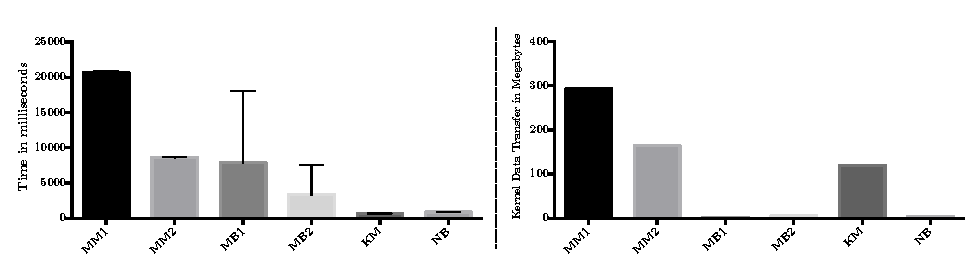
\includegraphics[width=1.0\textwidth]{images/benchmark_kernel_data_transfers.pdf}
	\centering
	\caption{Average Benchmark Partial Runtimes and Data Transfer Sizes}
	\label{img:benchmark_kernel_attributes}
\end{figure}

While it is visible that the computation times are significantly different, it can also be seen that the respective data transfers do not correlate to that attribute. For example, while MM2 and MB1 may require similar execution times, MM2 transfers 100x more data than MB1. The same is true for the iterative jobs KM and NB. It must be noted that MB1 and MB2 show high standard deviations, which are not measurement errors but are a result of the nature of the algorithm. Mandelbrot calculations can not be split evenly in terms of computational effort and instead may run some partials for long times while having virtually no computations required by other partials.

For the benchmark, the relevant performance indicator to measure were the total wall clock time to finish all jobs. As the selection of scheduling algorithms has a big impact on this value, it was necessary to define the utilized algorithms. For the job scheduling tier, the \textit{Round-Robin} approach was used. On the device scheduling level, the historic \textit{Performance Based Device Scheduler} was selected, which assigns a partial to the best suiting device in case multiple devices are available. In order to allow for a fair comparison among multiple runs, all jobs were submitted before starting the \textit{Job Executor}.

\section{Local Distribution}
\label{local_distribution}
A possible use case of Dynamic OpenCL is the outsourcing of entire computations to remote machines without allowing participation of the host machine itself. Such a setup is hereby defined as a \textit{Fully Assisted Computation}. Executing a fully assisted computation might be meaningful due to severe differences in hardware capabilities between the host and the remote machines. For example, when a low powered ARM machine offloads workloads to a high-performance server, it is likely to be beneficial to not include the ARM machine in the computation as it may slow down the overall process.

The second conceived cluster setup is defined as a \textit{Partially Assisted Computation}. In it, the local cluster grants computational support to a machine that needs to finish a workload faster than it can achieve on its own. This is especially useful when certain deadlines have to be met but a single machine can not match the performance requirements.

\subsection{Fully Assisted Computation}
In this scenario that covers the fully assisted setup, a single machine of Type A acted as the management node that received the given jobs. In the first round, it was connected to a single execution node of Type B. The measured times of the benchmarks for the single execution node represent the performance baseline. Subsequently, the measurements were then repeated after adding more machines of Type B one by one.

\subsubsection*{Single Job Performance}

The benchmark results for the matrix multiplication in figure \ref{img:fully_assisted_parallel_matrix} display that the performance gains for the given cluster configuration are not on par with the actually available performance. The second remote machine can still yield speedups to around 1.5x for bigger problem sizes while the second machine only raises that value to around 1.7x. From there on every further cluster expansion yields minimal improvements to a maximum of 1.75x and in the case of the last machine even decreases performance. This behavior is the result of the 1 Gbit/s connection being such a narrow bottleneck that can not serve the participating machines adequately and thus keeps their CPUs idle for longer timespans.
\begin{figure}[!htb]

	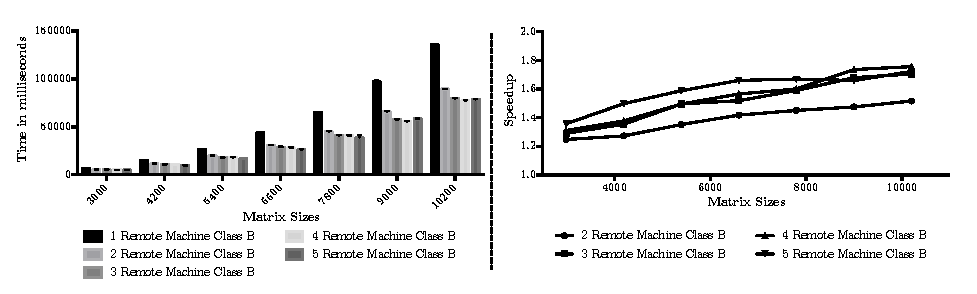
\includegraphics[width=1.0\textwidth]{images/local_fully_assisted_matrix.pdf}
	\centering
	\caption{Local Fully Assisted Parallel Matrix Multiplication}
	\label{img:fully_assisted_parallel_matrix}
\end{figure}

In the case of the Mandelbrot set the cluster performed much better as shown in figure \ref{img:fully_assisted_parallel_mandelbrot}. While the second machine can improve the performance by a near perfect speedup of around 1.9x, even the third and fourth machine can reproduce this behavior with a speedup 2.85x and 3.7x respectively. From the results, it can be inferred that the fifth machine saturates the performance for the given workload with a maximum speedup of 4.0x. A probable explanation for this barrier is the inequality in computational complexity among partials. This causes additional machines to remain idle for the majority of the time as not enough partials with longer computations are available.

\begin{figure}[!htb]

	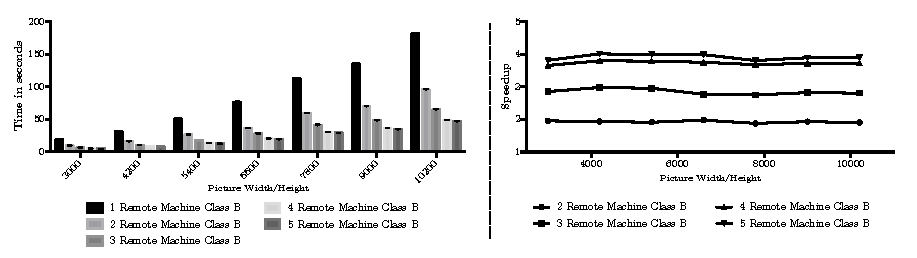
\includegraphics[width=1.0\textwidth]{images/local_fully_assisted_mandelbrot.pdf}
	\centering
	\caption{Local Fully Assisted Parallel Mandelbrot}
	\label{img:fully_assisted_parallel_mandelbrot}
\end{figure}
\subsubsection*{Job Suite Performance}

\begin{figure}[!htb]

	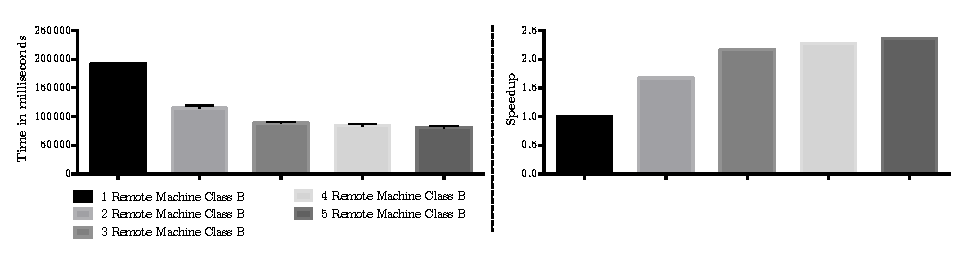
\includegraphics[width=1.0\textwidth]{images/local_fully_assisted_full_benchmark.pdf}
	\centering
	\caption{Local Fully Assisted Job Suite Benchmark Results}
	\label{img:local_fully_assisted_benchmark_results}
\end{figure}

The job suite benchmark, which can be seen in figure \ref{img:local_fully_assisted_benchmark_results}, implicates that the data-intensive jobs in it dominate the results for this cluster as the speedup values resemble those of the matrix multiplication. While the second and third machine can introduce a 1.7x and 2.2x speedup, every additional machine can only bring minuscule improvements. Once again more machines congest the network and thus do not benefit the cluster instead of increasing the computational performance.

\subsection{Partly Assisted Computation}

In order to simulate the use case of the partly assisted computation, the initial cluster setup was comprised of a single machine of Type B, which acted as the management node as well as an execution node. This node represents the performance baseline that serves for speedup comparisons. Then in each benchmark iteration, a remote node of Type B was added. Therefore all participating machines employed 10 Gbit/s connections with the central node having the potential bottleneck as it had to serve multiple equal connections. The setup also implicates that not all partials had to be transferred via network as some were computed directly on the central node.

\subsubsection*{Single Job Performance}
\label{single_job_performance}

\begin{figure}[!htb]

	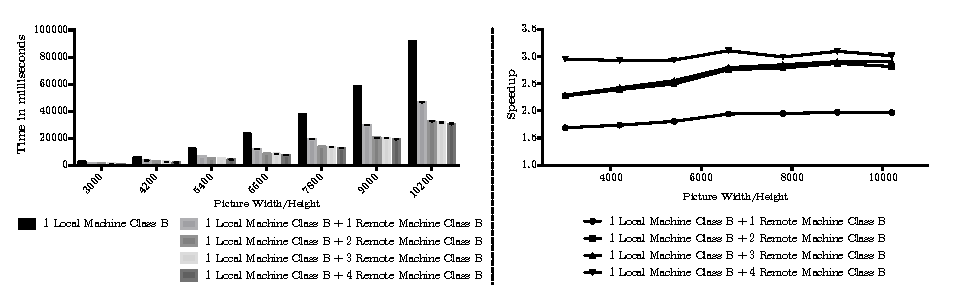
\includegraphics[width=1.0\textwidth]{images/local_partially_assisted_matrix.pdf}
	\centering
	\caption{Local Partially Assisted Parallel Matrix Multiplication}
	\label{img:parallel_matrix}
\end{figure}

Figure \ref{img:parallel_matrix} shows the results for the matrix multiplication. It identifies that using an additional machine can lead to substantial performance benefits. One can observe that with a single additional remote machine for small problem sizes the speedup is already significant with at least 1.65x speedup and reaches around 1.95x for bigger problem sizes. Adding a second remote machine benefits the cluster nearly as much as the first remote machine with speedups rising to around 2.8x for the biggest problem size. Introducing a third and fourth remote machine does not yield significant additional speedups as the number of splits is only six and therefore too low to effectively serve that many machines.

\begin{figure}[!htb]

	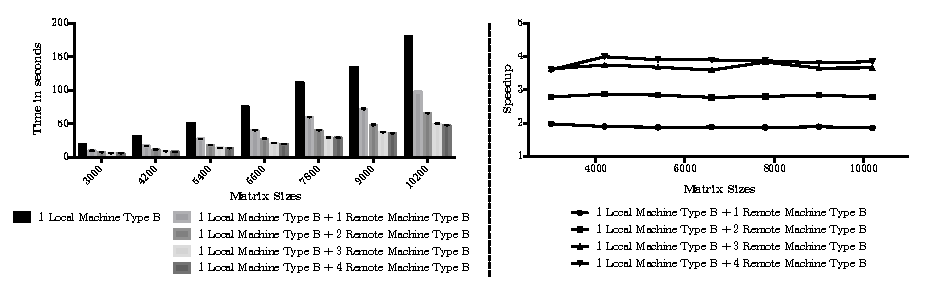
\includegraphics[width=1.0\textwidth]{images/local_partially_assisted_mandelbrot.pdf}
	\centering
	\caption{Local Partially Assisted Parallel Mandelbrot}
	\label{img:parallel_mandelbrot}
\end{figure}

Figure \ref{img:parallel_mandelbrot} reveals that in the case of the Mandelbrot set its low data transfer requirements severely benefit the performance speedup. With every added remote machine the speedup increases close to perfection for all problem sizes until the fourth remote machine is introduced to the cluster. Then the benefits are only minuscule because there are not enough compute-intensive splits available to saturate all participating machines efficiently. Thus, the maximum speedup for 3 remote machines is 3.8x while for 4 remote machines it is only lifted to 4.0x.


\subsubsection*{Job Suite Performance}
\label{job_suite_performance}

\begin{figure}[!htb]

	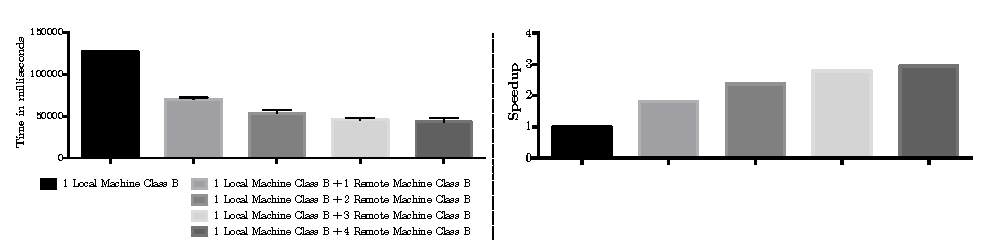
\includegraphics[width=1.0\textwidth]{images/local_partially_assisted_full_benchmark.pdf}
	\centering
	\caption{Local Partially Assisted Job Suite Benchmark Results}
	\label{img:local_benchmark_results}
\end{figure}

The results in figure \ref{img:local_benchmark_results} indicate that employing additional remote machines for mixed workloads can produce significant performance benefits. Especially the first and second remote machine yield a respective 1.8x and 2.4x speedup. The third and fourth machine can only add smaller performance improvements to around 2.8x and 3.0x speedup. The reason for the decreasing slope in performance increase could be the presence of symmetric network connections. With a higher amount of participating remote machines, the connection to the central node becomes more and more contested. Therefore every added node reduces the performance of the previously existing nodes in order to obtain its own share of bandwidth.


\section{Hybrid Distribution}

After having discussed the benefits of local workload distributions, it is necessary to evaluate the performance of Dynamic OpenCL when connected to cloud resources. A possible use case is represented by a situation in which available local machines can not provide sufficient performance to match the current requirements. Hence, employing remote cloud resources can be a meaningful option to gain additional computational potential for short periods of time. For this, the cluster initially held a single local machine of Type B. It served as a management node as well as an execution node. Its performance in the benchmarks is used as the baseline for comparisons. Then additional cloud resources were booked from the EC2 and added to the cluster. For the cloud resources, the high-performance instance type c4.8xlarge was chosen, which is described in section \ref{cluster_composition}.

While 10 Gbit/s connections are proven to be a potent solution when distributing among a local cluster, hybrid clusters suffer from far slower bottlenecks in between the two networks. The local cluster was set in Potsdam and therefore connected to the geographically closest region that was available on the EC2 cloud, which is Frankfurt. In order to prove the presence of a bottleneck, the connection speed between the two locations was measured by using iperf3 and ping from the Type B machine to a cloud machine over a minute. These results were then compared to the measured metrics from within the EC2, which are presented in section \ref{cluster_composition}. Although local EC2 bandwidths and latencies could reach promising values of 9.44 Gbit/s and 0.158 ms, accessing the same instances from a network outside the cloud only yielded 169.26 Mbit/s ($\sigma = 11.93$) and 18.9 ms ($\sigma = 0.17$). A reason for the low remote performance numbers could be bottlenecks within the local network that reduced the bandwidth significantly. In order to investigate this theory, three machines of type c4.8xlarge were started. Then the local machine launched iperf3 tests for 60 seconds in parallel to each of the three machines. The results are shown in figure \ref{img:EC2 Parallel Network Performance}.

\begin{figure}[!htb]
	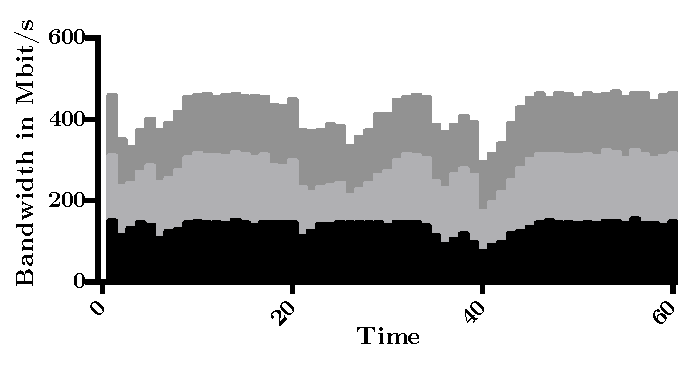
\includegraphics[width=0.5\textwidth]{images/ec2_stacked_network_performance.pdf}
	\centering
	\caption{EC2 Parallel Network Performance}
	\label{img:EC2 Parallel Network Performance}
\end{figure}

It is visible that the total network performance reached 480 MBit/s for some data points, which disproves that the local network was bottlenecked to the bandwidths of a single instance. In order to identify the limiting factor, the bandwidth to the EC2 was again measured from a different network in Berlin. From there average bandwidths of 306 MBit/s were achieved. This disproves that the EC2 itself limits the incoming connections. Still, from the machines within the Potsdam cluster downloading large files from other internet locations allowed bandwidths up to 360 MBit/s. Therefore it is concluded that during the routing from Potsdam to the EC2 the bandwidths were limited, which was not enforced on other routes.

\subsection*{Single Job Performance}

\begin{figure}[!htb]
	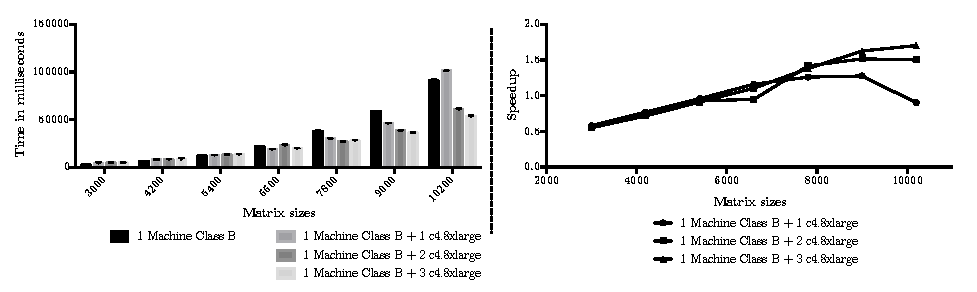
\includegraphics[width=1.0\textwidth]{images/hybrid_matrix_multiplication.pdf}
	\centering
	\caption{Hybrid Matrix Multiplication}
	\label{img:hybrid_matrix_multiplication}
\end{figure}

Figure \ref{img:hybrid_matrix_multiplication} displays the results for the matrix multiplications. It is visible that in the case of smaller problem sizes adding cloud devices slows down the process. With increasing sizes, the speedup factor grows but never reaches values that would match the actual hardware capabilities of the c4.8xlarge instances. This is due to the slow connection between both networks, which is much slower than the bus speeds of the c4.8xlarge. Therefore it mainly remains underutilized due to the increased transfer times. For a single cloud instance, the largest problem size causes an unexpected drop in performance, which can be explained by the cloud instance coincidentally picking the last available partial, thus making it run for a substantial timespan while the local instance has already finished all its partials. Adding more instances does not greatly enhance the performance but can provide a maximum speedup of 1.7x for three cloud instances.


\begin{figure}[!htb]
	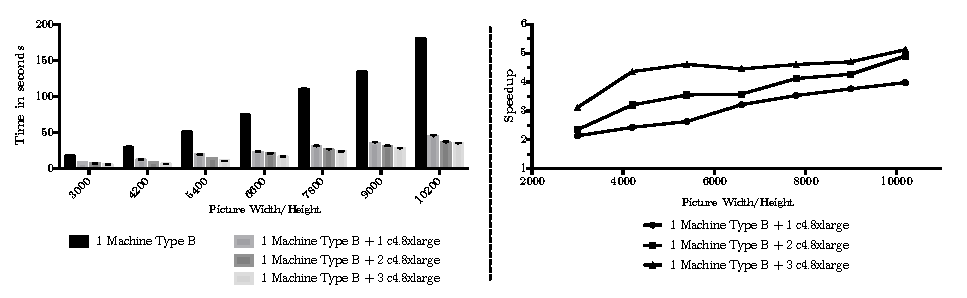
\includegraphics[width=1.0\textwidth]{images/hybrid_mandelbrot_performance.pdf}
	\centering
	\caption{Hybrid Mandelbrot Set}
	\label{img:hybrid_mandelbrot}
\end{figure}

For the second benchmark the Mandelbrot set was used again, which promises better performance than matrix multiplications on a hybrid setup due to its lower data requirements. The results of the measurements are shown in figure \ref{img:hybrid_mandelbrot}. In fact the c4.x8large can greatly improve the overall system performance through its 36 cores. Even for small problem sizes it already provides significant benefits but especially for the larger sizes it can speed up the execution by around 4x. Adding more machines yields some further improvements but not to the same extent as the first machine. The maximum observed speedup for three cloud instances therefore lies at around 5.1x.

From the results it can be concluded that the data requirements of a workload have an even greater impact on performance for hybrid setups than on an entirely local setup. For data heavy workloads, such as matrix multiplications, which have to transfer hundreds of megabytes of data, the hybrid setup can actually produce slowdowns instead of improving performance. In the case of jobs with little data the availability of high performance cloud resources may yield great benefits when assisting slower local hardware.

\subsection*{Job Suite Performance}

\begin{figure}[H]
	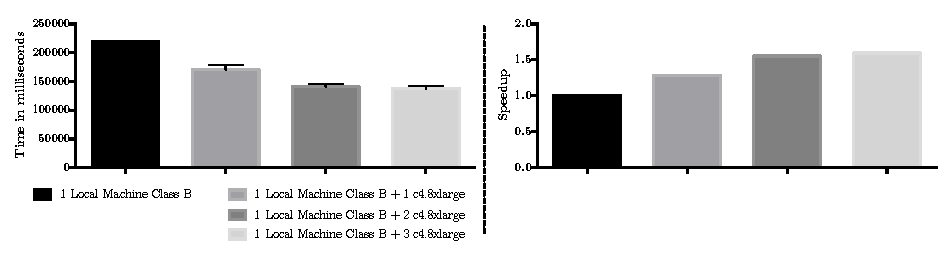
\includegraphics[width=1.0\textwidth]{images/hybrid_full_benchmark_performance_based.pdf}
	\centering
	\caption{Hybrid Job Suite Benchmark Results}
	\label{img:hybrid_benchmark_results}
\end{figure}

Figure \ref{img:hybrid_benchmark_results} shows the results of the benchmark for the hybrid cluster. It is visible that the performance benefits are quite insignificant in relation to the potential computational capability of the c4.8xlarge instance types. Scaling the cluster to two machines with one c4.8xlarge gives a 1.28x performance increase. Adding another c4.8xlarge instance grants an overall 1.55x faster execution compared to the single local machine. When a third instance is introduced, it becomes obvious that a barrier is hit for this benchmark as the speedup compared to two cloud machines is minimal. As shown earlier, the EC2 offers low network bandwidth when accessed by the local cluster. While the performance based scheduler can take these factors into account through its history based approach it still has to run a partial of a job at least once to gain a performance measurement. Therefore it is common that partials with big data transfers are assigned to cloud machines, thus resulting in slow execution times for these kernels.

In order to optimize the assignment of data-intensive jobs to the appropriate devices, a new scheduler was built that has awareness of the different network locations. For this, all available devices are marked whether they are originating from the local cluster or the cloud provider. The scheduler then ignores the partial order given by the first scheduling tier, e.g.~Round-Robin, and imposes its own order. In fact, it sorts the assignable partials by the amount of data they comprise and assigns them from either end of the list: cloud devices receive partials with little data while local devices are assigned those with the biggest data sizes. Hence, partials should reach cloud devices much faster and the scheduling is not reliant on historical data anymore. With the new scheduler, the benchmark was repeated.

\begin{figure}[!htb]
	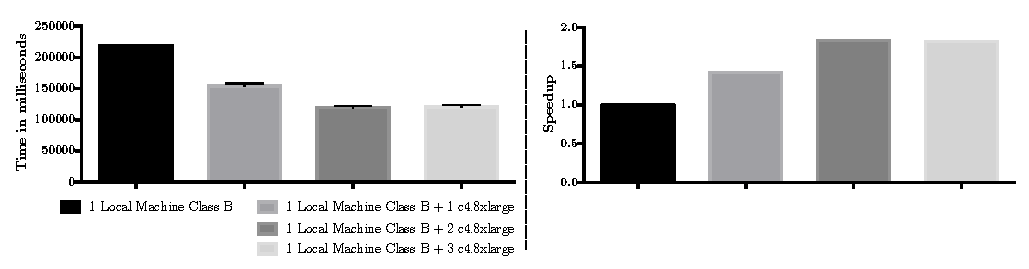
\includegraphics[width=1.0\textwidth]{images/hybrid_full_benchmark_network_based.pdf}
	\centering
	\caption{Hybrid Job Suite  Benchmark Results (Network Aware Scheduler)}
	\label{img:hybrid_benchmark_results_network_aware}
\end{figure}

Figure \ref{img:hybrid_benchmark_results_network_aware} shows that the new scheduler introduces noticeable benefits compared to the historical performance based approach. While a single c4.8xlarge instance improves the system performance by 1.42x, adding another one leads to a 1.83x increase. Compared to 1.28x and 1.55x respectively for the performance based scheduler, this depicts a significant improvement even though the new mechanism is not sophisticated. When a third c4.8xlarge machine is introduced to the cluster, no further speedup can be achieved. This can be reasoned by a too low number of jobs with small data transfers within the job suite to match the speed of the three cloud instances.

In order to prove that Dynamic OpenCL can deal with a multitude of different small data jobs in parallel, a second job suite was specified. For this, six Mandelbrot sets and four n-body computations of different sizes were used that have average kernel runtimes between 360 milliseconds and 8.5 seconds on a machine of Type B. The data sizes per kernel were in the range between 0.75 megabytes and 7 megabytes. Figure \ref{img:low_data_benchmark_statistics} shows the average runtimes on the Type B machine and data transfer sizes per partial.

\begin{figure}[!htb]
	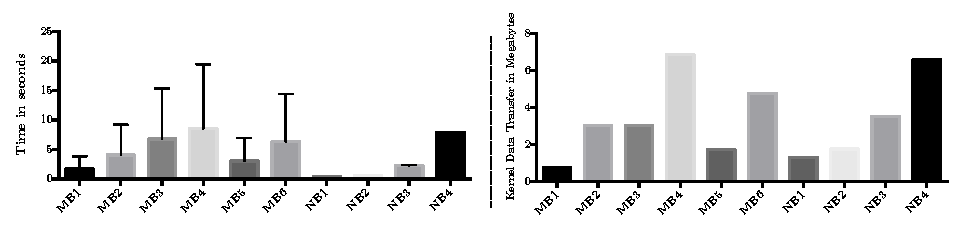
\includegraphics[width=1.0\textwidth]{images/lowdata_benchmark_statistics.pdf}
	\centering
	\caption{Low Data Job Suite Benchmark Kernel Runtimes and Data Transfer Sizes}
	\label{img:low_data_benchmark_statistics}
\end{figure}

The newly defined job suite was run on the same hybrid cluster as the previous mixed job suite. Again the network aware scheduler was used as transferring the kernels with 7 megabytes was expected to require around half a second when sent to the cloud.

\begin{figure}[!htb]
	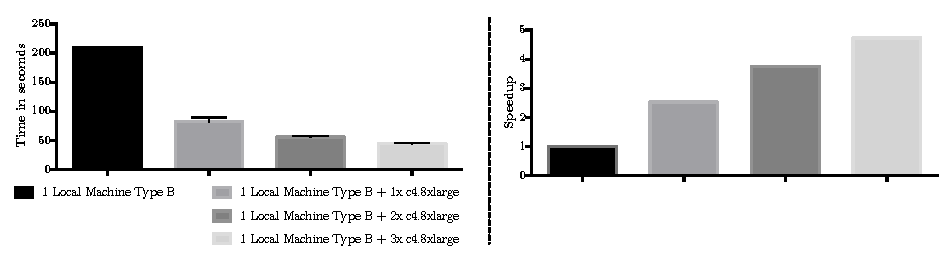
\includegraphics[width=1.0\textwidth]{images/hybrid_lowdata_benchmark.pdf}
	\centering
	\caption{Hybrid Low Data Job Suite Benchmark Results (Network Aware Scheduler)}
	\label{img:hybrid_low_data_benchmark_results_network_aware}
\end{figure}

Figure \ref{img:hybrid_low_data_benchmark_results_network_aware} shows that the cloud resources indeed can greatly improve performance for a job suite with low data requirements. With a 2.5x, 3.7x and 4.7x speedup every added c4.8xlarge instance benefits the overall computation time and thus can support the local machine with its partials. This is possible because the 36 core CPUs are better utilized in this scenario and their potential is not slowed down by expensive network transfers.

\section{Cloud Distribution}

In this scenario, all utilized resources were located at a cloud service like Amazon's EC2. One central management node was run that does not execute any computations but distributes the partials instead. The instance type for the management node was chosen based on the availability of a 10 Gbit/s connection, which was the c4.8xlarge type. For the actual computations, two different cluster sets were used. First, all benchmarks were run on a CPU cluster that was comprised of a varying number of c4.8xlarge instances. Then all tests were run again on g2.2xlarge instances, which provided a NVIDIA GRID K520 GPU.

\subsection{CPU Cluster}
\subsubsection*{Single Job Performance}

Figure \ref{img:ec2_cpu_matrix_multiplication} shows the performance of the CPU cluster for the matrix multiplications. As soon as a second instance is added to the cluster it is visible that the performance increases significantly but imperfectly as the instances now have to share the network. Therefore perfect scaling is impossible but nevertheless the second instance can provide a maximum speedup of around 1.9x for the largest problem size. The third instance once again reduces the overall computation time, peaking at around 2.8x.

\begin{figure}[!htb]
	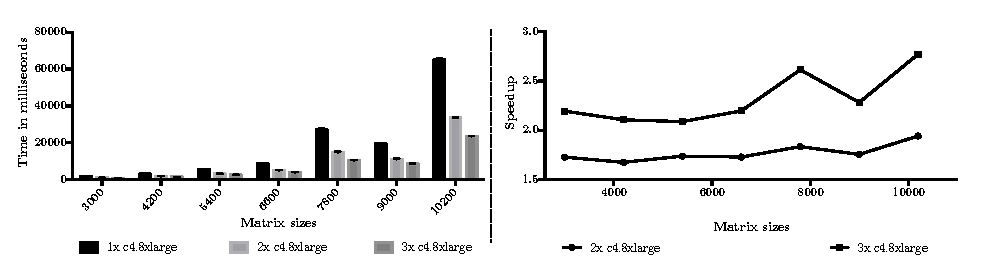
\includegraphics[width=1.0\textwidth]{images/ec2_cpu_matrix_multiplication.pdf}
	\centering
	\caption{EC2 Pure Cloud Matrix Multiplication on CPUs}
	\label{img:ec2_cpu_matrix_multiplication}
\end{figure}

It must be noted that the problem sizes 7800 and 9000 seem to produce an anomaly for this instance type as the larger size actually leads to shorter computation times. This appears to be a particularity of the c4.8xlarge instances as it could not be observed with any other tested hardware.


\begin{figure}[!htb]
	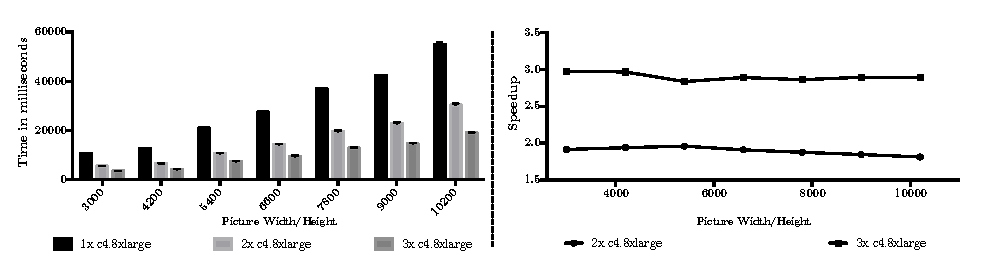
\includegraphics[width=1.0\textwidth]{images/ec2_cpu_mandelbrot.pdf}
	\centering
	\caption{EC2 Pure Cloud Mandelbrot Set on CPUs}
	\label{img:ec2_cpu_mandelbrot}
\end{figure}

In figure \ref{img:ec2_cpu_mandelbrot} the performance of the cluster for the Mandelbrot set is displayed. Unlike the matrix multiplications, the observed performance improvements are high for all problem sizes and peak at 1.96x for two instances and 2.97x for three instances. Once again the benefits of a 10 Gbit/s connection can be proven even though it is shared among the three participating machines.
\subsubsection*{Job Suite Performance}

\begin{figure}[!htb]
	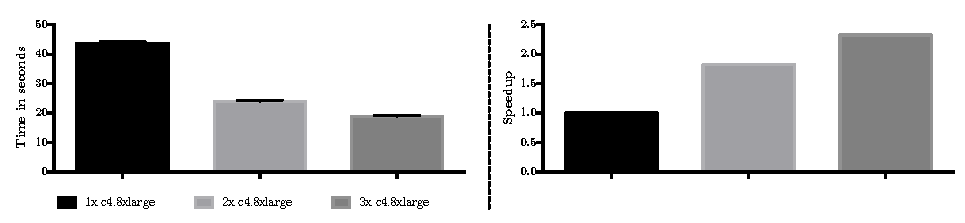
\includegraphics[width=1.0\textwidth]{images/ec2_cpu_full_benchmark.pdf}
	\centering
	\caption{EC2 Pure Cloud Job Suite Benchmark on CPUs}
	\label{img:ec2_cpu_full_benchmark}
\end{figure}

Figure \ref{img:ec2_cpu_full_benchmark} shows the performance of the CPU cluster for the job suite benchmark. It can be inferred that the performance gains of a second instance are substantial at a 1.8x speedup even though the benchmark contains several data heavy jobs. Indeed employing three instances yields another boost in computational power, providing a 2.3x speedup. Still, it is visible that the gains of the third instance do not match those of the second as more machines have to compete for network resources.

\subsection{GPU Cluster}
\subsubsection*{Single Job Performance}

\begin{figure}[!htb]
	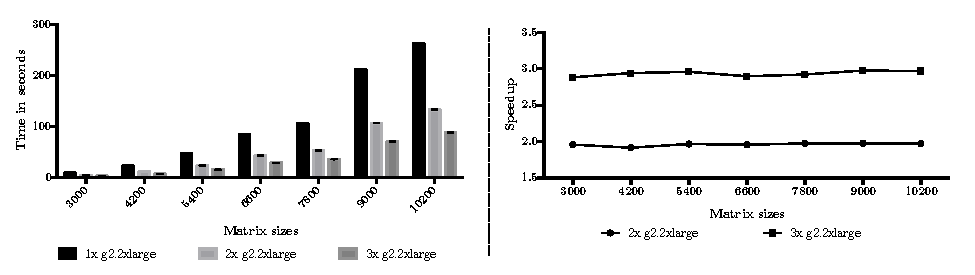
\includegraphics[width=1.0\textwidth]{images/ec2_gpu_matrix_multiplication.pdf}
	\centering
	\caption{EC2 Pure Cloud Matrix Multiplication on GPUs}
	\label{img:ec2_gpu_matrix_multiplication}
\end{figure}

In figure \ref{img:ec2_gpu_matrix_multiplication} the benchmark results for the matrix multiplication are displayed. It is visible that there is a clear difference towards the CPU results as the speedup is nearly linear for all tested problem sizes. While this may surprise at first, the reason for this effect are the 1 Gbit/s connections of the GPU nodes that can not bottleneck the 10 Gbit/s connection of the management node. Therefore each additional node can introduce the same speedup until the connection of the management node is saturated, which in this case would probably happen after around 10 GPU instances.

\begin{figure}[!htb]
	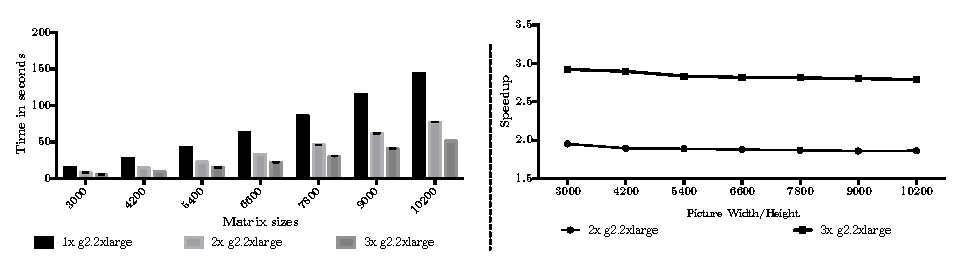
\includegraphics[width=1.0\textwidth]{images/ec2_gpu_mandelbrot.pdf}
	\centering
	\caption{EC2 Pure Cloud Mandelbrot Set on GPUs}
	\label{img:ec2_gpu_mandelbrot}
\end{figure}

The Mandelbrot set benchmarks, which can be seen in figure \ref{img:ec2_gpu_mandelbrot}, paint a similar picture. Whether two or three instances are used appears to be irrelevant in terms of additional speedup. Both machines can introduce almost linear performance benefits to the cluster as the data sizes are small and the 1 Gbit/s connections of all participating instances can be fully saturated.

\subsubsection*{Job Suite Performance}
Figure \ref{img:ec2_gpu_full_benchmark} shows the performance of the GPU cluster for the mixed job suite benchmark. Both the second and third GPU instance introduce a substantial performance increase to the cluster, with a 1.8x speedup and 2.5x speedup respectively.

\begin{figure}[!htb]
	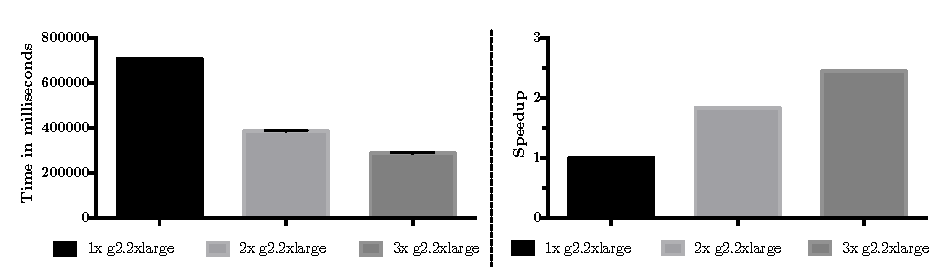
\includegraphics[width=1.0\textwidth]{images/ec2_gpu_full_benchmark.pdf}
	\centering
	\caption{EC2 Pure Cloud Job Suite Benchmark on GPUs}
	\label{img:ec2_gpu_full_benchmark}
\end{figure}
